\section{Use cases satisfaction: entities interactions}\label{use_cases_satisfaction}
This section will show how the entities introduced in the Architecture just presented actually cooperate with each other in order to satisfy the use cases previously discussed in \textit{section \ref{use_cases}}. 

\subsection{Contributor}
\begin{itemize}
    \item \textbf{Register}\\
    \begin{figure}[!ht]
        \centering
        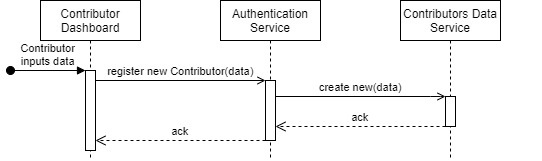
\includegraphics[scale=1]{document/chapters/chapter_6/images/use_cases_satisfaction_contributor_register.jpg}
        \caption{Contributor registration}
        \label{fig:use_cases_satisfaction_contributor_register}
    \end{figure}

    A Contributor registers to the Grid system creating an account using the Contributor Dashboard; once it has inputted the necessary data, the Dashboard will contact the Authentication with the dedicated API that, in turn, will contact the Contributors Data Service, actually completing the registration process.

    \item \textbf{Login}\\
    When a Contributor performs a Login, both in the Dashboard case and in the Contributing Endpoint, it gets a token that will be used for every subsequent operation for both authenticating the communication with other entities and, at the same time, provide some useful data that will be used by said entities.
    
    Since the token is a prerequisite for every further interaction it will be omitted for simplicity in the subsequent single use case satisfaction discussions. 
     
    \begin{itemize}
        \item \textbf{\textit{Login to a Dashboard}}\\
        \begin{figure}[!ht]
            \centering
            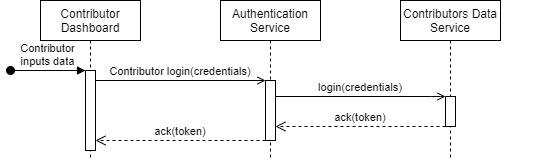
\includegraphics[scale=1]{document/chapters/chapter_6/images/use_cases_satisfaction_contributor_dashboard_login.jpg}
            \caption{Contributor Dashboard login}
            \label{fig:use_cases_satisfaction_contributor_dashboard_login}
        \end{figure}

        The login process performed by a Dashboard is very similar to the registration one, diverging only in the invocation of a different specific API.
        \vspace{4mm}

        \item \textbf{\textit{Login from any Contributing Endpoint able to Contribute}}\\
        \begin{figure}[!ht]
            \centering
            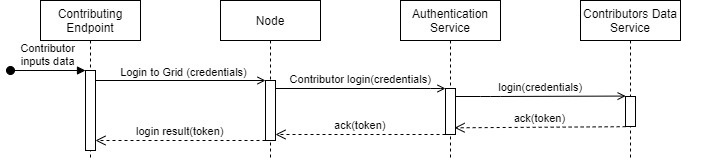
\includegraphics[scale=0.8]{document/chapters/chapter_6/images/use_cases_satisfaction_node_login.jpg}
            \caption{Node login}
            \label{fig:use_cases_satisfaction_node_login}
        \end{figure}

        Here, the Contributor Application is the one actually triggering the Login in its integrated Node; then, the Node's login differs from the Dashboard'one calling another dedicated API that also require to provide some additional info that will uniquely identify the device.
        
        The Customer only needs to make the active effort of registering its account; every Contributing Endpoint will be automatically added to its account if the credentials are correct and no matching device for its account is found.
        One important thing to notice is that the token does not exit the Node's scope.

    \end{itemize}

    \item \textbf{Passively Contribute offering a compatible device}\\
    \begin{figure}[!ht]
        \centering
        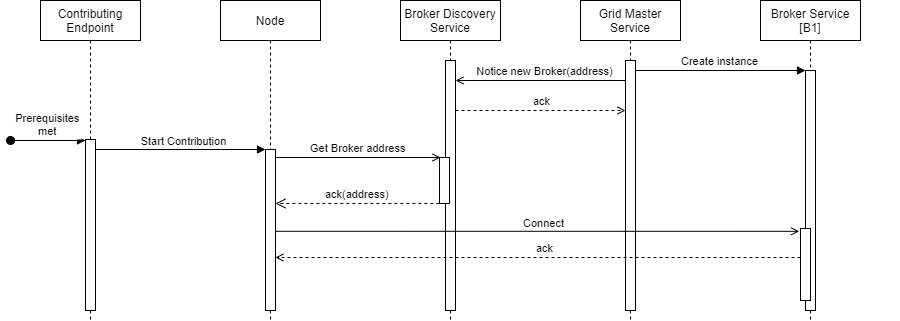
\includegraphics[width=\linewidth]{document/chapters/chapter_6/images/use_cases_satisfaction_node_grid_connection.jpg}
        \caption{Connection to the Grid}
        \label{fig:use_cases_satisfaction_node_grid_connection}
    \end{figure}

    \begin{figure}[!ht]
        \centering
        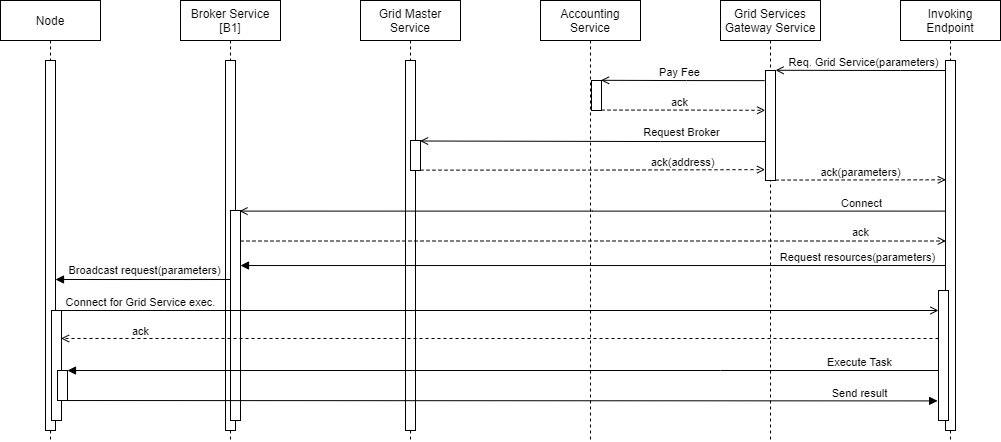
\includegraphics[width=\linewidth]{document/chapters/chapter_6/images/use_cases_satisfaction_node_contribution.jpg}
        \caption{Node Contribution}
        \label{fig:use_cases_satisfaction_node_contribution}
    \end{figure}

    \begin{itemize}
        \item \textit{Accumulate Rewards}\\
        \begin{figure}[!ht]
            \centering
            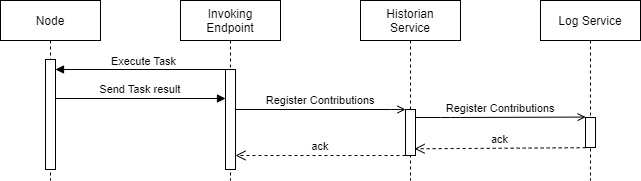
\includegraphics[scale=0.65]{document/chapters/chapter_6/images/use_cases_satisfaction_rewards_accumulation.jpg}
            \caption{Rewards accumulation}
            \label{fig:use_cases_satisfaction_rewards_accumulation}
        \end{figure}
        \item \textit{Manually start/stop Contribution from the Contributing Endpoint}\\
        % no need for diagram
        \item \textit{Configure Access Policies to the Contributing Endpoint's Resources}\\
        % no need for diagram
        \item \textit{Check if Contributing Endpoints are currently Contributing}\\
        % no need for diagram
    \end{itemize}
    \item \textbf{Manage Contribution data through a Dashboard}\\
    \begin{itemize}
        \item \textit{Check past Contributions}\\
        \begin{figure}[!ht]
            \centering
            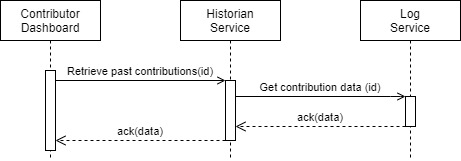
\includegraphics[scale=0.65]{document/chapters/chapter_6/images/use_cases_satisfaction_past_contributions_check.jpg}
            \caption{Contributor's past Contributions check}
            \label{fig:use_cases_satisfaction_past_contributions_check}
        \end{figure}
        \item \textit{Check Rewards Balance}\\
        \begin{figure}[!ht]
            \centering
            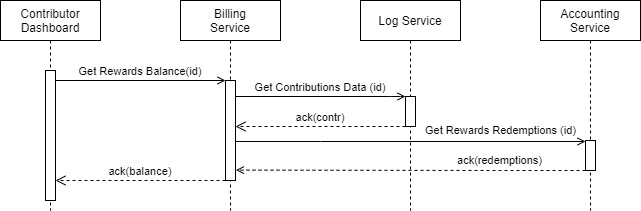
\includegraphics[scale=0.65]{document/chapters/chapter_6/images/use_cases_satisfaction_rewards_balance.jpg}
            \caption{Contributor's Rewards Balance check}
            \label{fig:use_cases_satisfaction_rewards_balance}
        \end{figure}
        \item \textit{Rewards Redemption}\\
        \begin{figure}[!ht]
            \centering
            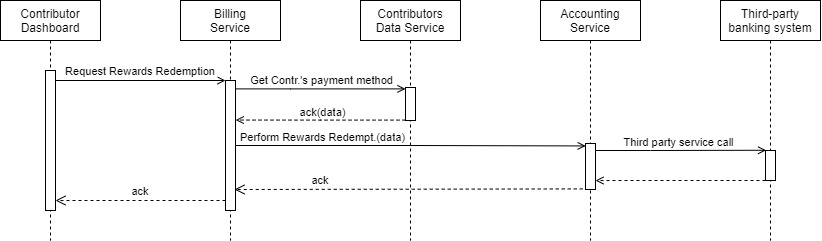
\includegraphics[width=\linewidth]{document/chapters/chapter_6/images/use_cases_satisfaction_rewards_redemption.jpg}
            \caption{Contributor's Rewards Redemption}
            \label{fig:use_cases_satisfaction_rewards_redemption}
        \end{figure}
    \end{itemize}
\end{itemize}

\subsection{Customer}
TODO

\begin{itemize}
    \item \textbf{Register}\\
    \item \textbf{Login}\\
    \begin{itemize}
        \item \textit{Login to a Dashboard}\\
        \item \textit{Authenticate for Grid Services Invocations}\\
    \end{itemize}
    \item \textbf{Easily integrate the Invoking Endpoint in a Customer Custom Application}\\
    \begin{itemize}
        \item \textit{Invoke Grid Services through any Device}\\
        \item \textit{Request MapReduce service}\\
        \begin{itemize}
            \item Define MapReduce data source\\
            \item Define Resource quantity to use\\
            \item Define Map and Reduce functions\\
        \end{itemize}
    \end{itemize}
    \item \textbf{Manage requested Grid Services data through a Dashboard}\\
    \begin{itemize}
        \item \textit{Check Grid Services Invocations history}\\
        \item \textit{Check running Grid Services Invocations}\\
        \item \textit{Check past Grid Services Invocations Fees}\\
        \item \textit{Manage payment methods}\\
    \end{itemize}
\end{itemize}